%% Преамбула TeX-файла

% 1. Стиль и язык
\documentclass[utf8x, 12pt]{G7-32} % Стиль (по умолчанию будет 14pt)

% Остальные стандартные настройки убраны в preamble.inc.tex.
\include{preamble}

\begin{document}

% выключает нумерацию ВСЕГО;
% здесь начинаются ненумерованные главы:
% реферат, введение, глоссарий, сокращения и прочее.
\frontmatter

\begin{center} 

\large Санкт-Петербургский государственный университет

\large Математическое обеспечение и администрирование
информационных систем \\[5.5cm] 

\Large Глушень Павел Владимирович \\[0.6cm]

\huge Реализация редизайна главного экрана
приложения «Яндекс — с Алисой» \\[0.6cm]

\large Отчет по учебной практике (черновик)\\[3.7cm]


\end{center} 

% \begin{flushright}
% Научный руководитель: \\
% ... \\
% \end{flushright}


\vfill 

\begin{center} 
\large Санкт-Петербург \\ 2019
\end{center} 

\thispagestyle{empty}
\tableofcontents
\Introduction

Android-приложение «Яндекс — с Алисой» предоставляет доступ ко множеству
сервисов компании «Яндекс» — одной из крупнейших IT-компаний России.
По~мере развития и внедрения все новых и новых сервисов
появляется необходимость переосмысливать пользовательский интерфейс
приложения, делая его более современным и более удобным для пользователя.

В данном отчете пойдет речь об основном компоненте главного экрана
Android-приложения «Яндекс — с Алисой».
Для удобства, здесь и далее этот компонент будет называться Бендером\footnote{
    По легенде, в ранних версиях приложения элементы этого компонента
    вместе напоминали глаза и рот робота Бендера —
    персонажа мультсериала «Футурама» студии «20th Century Fox».
}.
Цель работы — реализация Бендера
с новым дизайном (см. рис.~\ref{fig:2-bender-compare}).

\begin{figure}[h]
    \center{\includegraphics[scale=0.25]{2-bender-compare}}
    \caption{Слева версия до редизайна, справа — после}
    \label{fig:2-bender-compare}
\end{figure}


\mainmatter

\chapter{Постановка задачи}
\label{cha:ch_1}

Целью работы является реализация нового Бендера, включая его схлопывание
(см. рис.~\ref{fig:3-1-shrink}). Требуется:

\begin{enumerate}
    \item Разработать архитектуру для нового Бендера:
    \begin{enumerate}
        \item Декомпозировать задачу,
        \item Описать базовый макет,
        \item Описать архитектуру компонента;
    \end{enumerate}
    \item Реализовать новый Бендер, решив каждую подзадачу,
    появившуюся в результате декомпозиции.
\end{enumerate}

\begin{figure}[h]
    \center{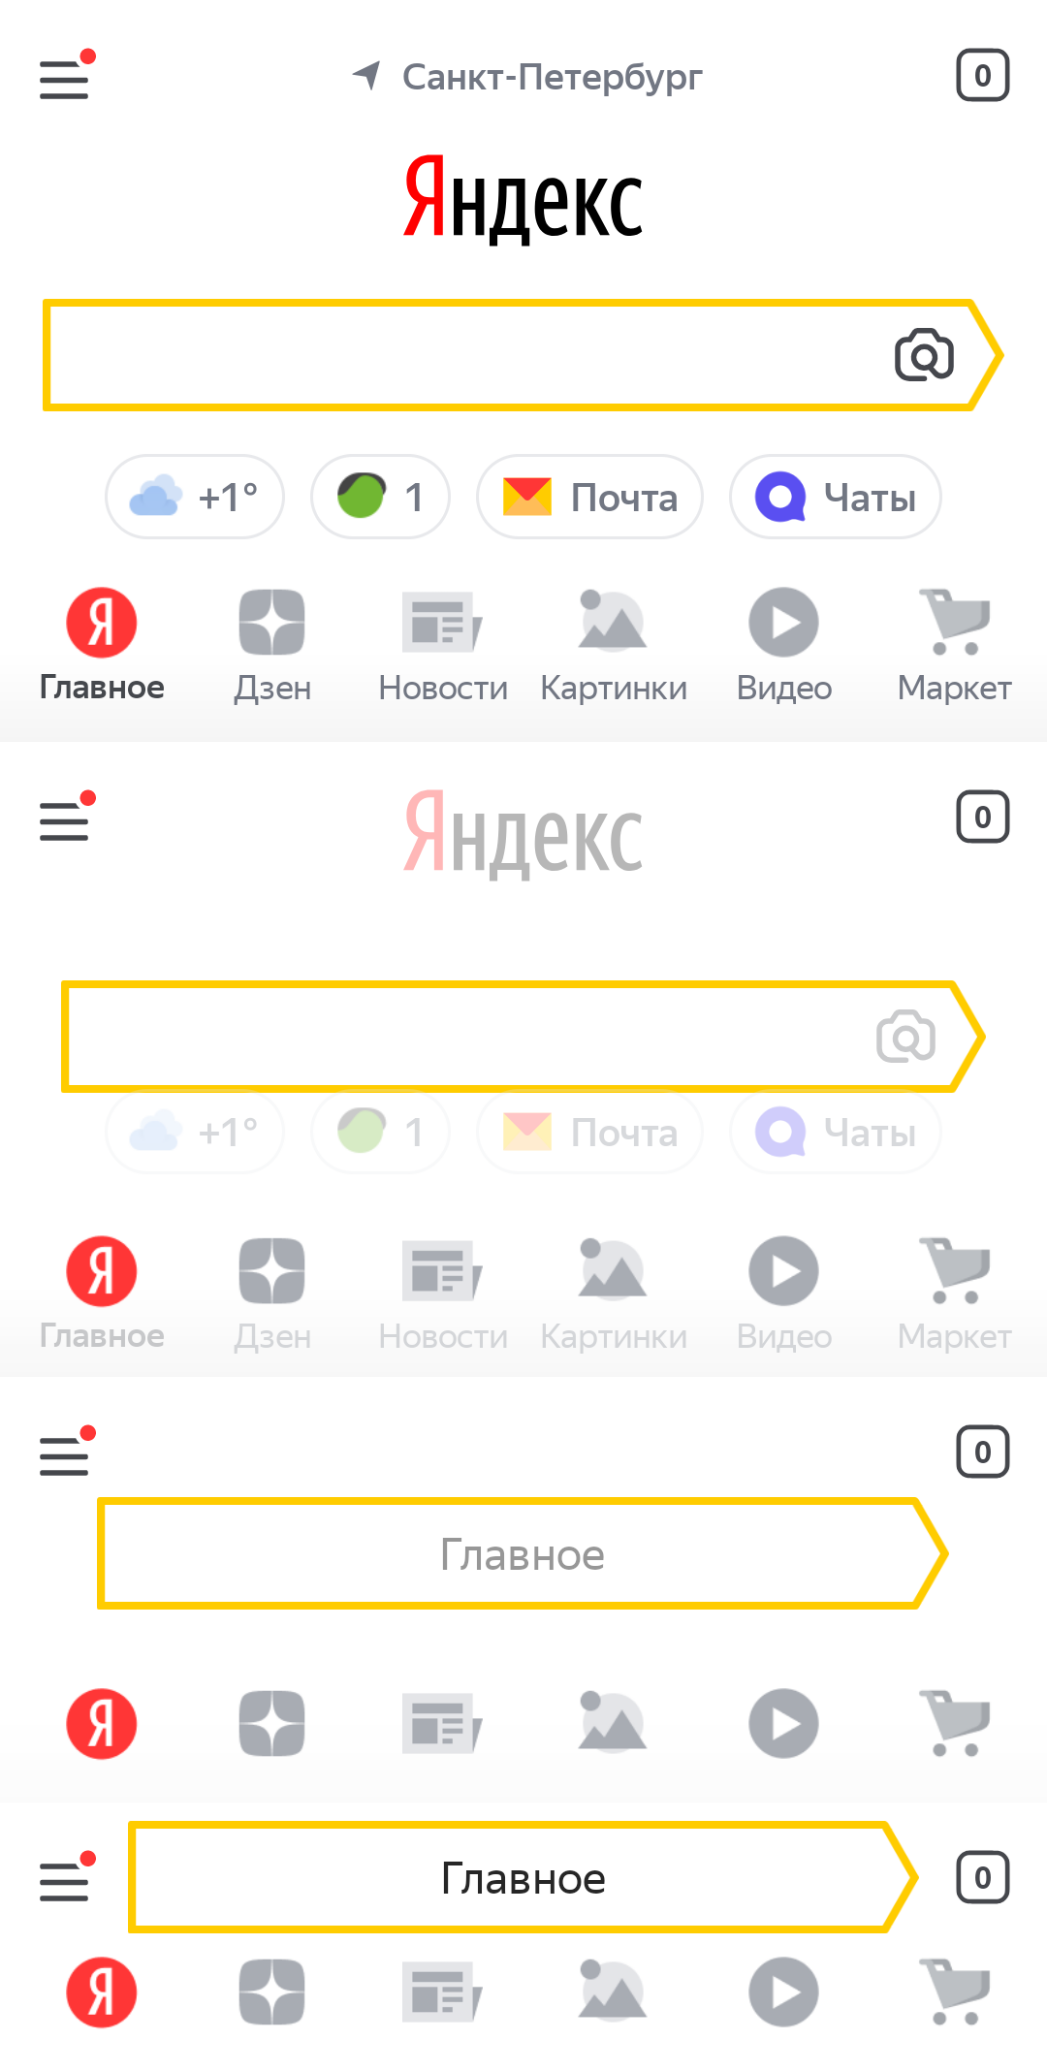
\includegraphics[scale=0.3]{3-1-shrink}}
    \caption{Процесс схлопывания Бендера}
    \label{fig:3-1-shrink}
\end{figure}

\chapter{Разработка архитектуры}
\label{cha:ch_2}

Для начала декомпозируем задачу. Нужно реализовать:
\begin{enumerate}
    \item Кнопку меню;
    \item Строку местоположения;
    \item Счетчик количества открытых браузерных вкладок;
    \item Логотип, который может превращаться в дудл;
    \item Омнибокс с кнопкой камеры;
    \item Информеры погоды, дорожного трафика, почты и чатов;
    \item Вкладки сервисов.
\end{enumerate}

Теперь нам нужно разработать базовый макет, расположив все эти элементы на нем.

Для начала заметим, что некоторые элементы можно сгруппировать таким образом,
чтобы получившиеся группы были расположены вертикально друг за другом.
Такая группировка позволяет нам использовать в качестве корневого элемента макета
LinearLayout — контейнер, распологающий элементы подряд вертикально или горизонтально.

Сгруппированные вместе кнопку меню, строку местоположения
и счетчик количества браузерных вкладок поместим во вложенный LinearLayout,
расположив элементы горизонтально друг относительно друга.
С информерами поступим так же.

Описав такую верстку в xml-файле, мы получаем возможность во время исполнения приложения
долучить дерево объектов, каждый из которых унаследован от класса View.
Объекты класса View представляют из себя элементы, отвечающие за отображение данных пользователю.

Для каждого из элементов нужно будет написать свою логику обновления данных
и реагирования на события, порожденные пользователем.
Для этого заведем класс BenderViewHolder, с которым будем взаимодействовать,
который будет взаимодействовать с обертками над внутренними компонентами.

\chapter{Реализация компонента}
\label{cha:ch_3}

\section{Кнопка меню}

В верстке используем \texttt{ImageView}, предназначенную для отображения
иконок~\cite{ImageView}.
В \texttt{BenderHamburgerViewHolder} поддерживаем два состояния:
с красной точкой и без нее.
Устанавливаем иконку в зависимости от указываемого состояния.
Кроме того, позволяем снаружи подписываться на событие клика
по~\texttt{ImageView}.

\section{Строка статуса}

В верстке используем \texttt{TextView}, позволяющий отображать текст
и иконки вокруг текста~\cite{TextView}.
В \texttt{BenderStatusTextViewHolder} поддерживаем два состояния:
онлайн и офлайн.
В онлайн-состоянии слева от текста проставляем иконку-стрелку,
текст меняем на название города, передаваемого при переходе в это состояние.
В~офлайн-состоянии проставляем иконку с изображением восклицательного знака
и текст \mbox{«Нет подключения к сети»}.
Позволяем снаружи подписаться на событие клика в онлайн-состоянии,
чтобы пользователь мог вручную изменить город.

\section{Счетчик браузерных вкладок}

В верстке используем \texttt{TextView} для отображения количества
открытых вкладок.
В \texttt{BenderBrowserTabCounterViewHolder} поддерживаем изменение числа
и позволяем снаружи подписываться на событие клика.

\section{Логотип}

В верстке используем \texttt{ImageView}.
Из \texttt{BenderLogoAndDoodleViewHolder} по умолчанию устанавливаем логотип
в качестве картинки, но позволяем менять ее снаружи.
Позволяем снаружи подписываться на событие клика.

\section{Омнибокс}

В верстке для самого омнибокса используем контейнер \texttt{FrameLayout},
позволяющий размещать элементы независимо друг от друга~\cite{FrameLayout}.
Устанавливаем ему фон, внутрь кладем \texttt{ImageView} для кнопки камеры
и \texttt{TextView} для названия текущего экрана в схлопнутом состоянии.
В \texttt{BenderOmniboxViewHolder} позволяем подписываться на события
клика по омнибоксу и по кнопке камеры.

\section{Информеры}

В верстке для информера используем \texttt{LinearLayout},
внутрь которого кладем \texttt{ImageView} для иконки
и \texttt{TextView} для текста.
В \texttt{BenderInformerViewHolder} поддерживаем изменение иконки и текста,
позволяем подписываться на события клика.
Элементы верстки для каждого информера складываем в общий для них
контейнер \texttt{LinearLayout} с горизонтальной ориентацией.

После этого для каждого конкретного информера создаем свой класс,
в который помещаем логику установки иконки и текста.
Этим классам делегируем логику через \texttt{BenderInformerContainerViewHolder}.

\section{Вкладки сервисов}

В верстке отдельной вкладки используем \texttt{LinearLayout},
внутрь него кладем \texttt{ImageView} для иконки и \texttt{TextView} для текста.
В \texttt{BenderTabViewHolder} поддерживаем два состояния:
активное с~яркой иконкой и жирным текстом
и неактивное с~черно-белой иконкой и обычным текстом.
Также позволяем подписываться на события клика.

После этого вкладки нужно поместить в контейнер со специфической логикой.
Контейнер должен запрашивать у каждого элемента, который в нем лежит,
размер минимальной ширины, которую этот элемент должен занимать,
после этого проставлять такой размер всем элементам,
чтобы ширина каждого элемента была одинаковой.
При этом, если не все элементы помещаются на экран,
то контейнер должен скроллиться.
А если помещаются, то поместить их нужно в центре контейнера.

Готового такого контейнера нет, но можем реализовать свой~\cite{CustomView}.
Им становится \texttt{BenderTabLayoutSlidingStrip} — унаследованный
от \texttt{ViewGroup} — предка всех контейнеров — контейнер,
поддержавший всю описанную выше логику, за исключением скроллинга.
Его помещаем внутрь \texttt{HorizontalScrollView},
который, как следует из его названия, и поддерживает нужный скроллинг.
При~наследовании переопределяем метод \texttt{onMeasure}, вычисляющий
высоту и ширину контейнера по его элементам, а также метод \texttt{onLayout},
вычисляющий координаты для размещения каждого элемента.

Логику наполнения элементами \texttt{BenderTabLayoutSlidingStrip}
и управления их состояниями размещаем в~\texttt{BenderTabLayoutViewHolder}.
Позволяем подписываться снаружи на клики по элементам
(при клике сообщаем индекс элемента, на который кликнули).

\section{Анимация схлопывания}

При схлопывании нам известен коэффициент слопывания — вещественное число,
равное 0 для расхлопнутого и 1 для полностью схлопнутого Бендера.
С помощью него мы рассчитываем коэффициент непрозрачности, смещение
и размеры изменяющихся элементов, после чего применяем их
к соответствующим элементам.


%% Здесь заканчивается нумерованная часть документа
%% и начинаются ссылки и заключение
\backmatter

\Conclusion

Для решения задачи она была сначала декомпозирована,
был описан базовый макет и структура классов.
После были решены возникшие подзадачи:
реализована кнопка меню, строка статуса, счетчик количества браузерных вкладок,
логотип, омнибокс с кнопкой камеры,
информеры погоды, дорожного трафика, почты и чатов, вкладки сервисов.
Кроме того, была реализована анимация схлопывания.


\include{5-biblio}

\end{document}
